% ::setlocal makeprg=cd\ presentazione\ &&\ pdflatex\ -interaction=batchmode\ main.tex\ &&\ xdg-open\ main.pdf\ &

\section{Capitolo 2}

\begin{frame}{Simulazione}

    Equazioni del moto per una particella massiva (unità adimensionali)

	\begin{align*}[left = {\empheqlbrace}]
        &\dv{\hat r}{\hat \tau} = \pm \sqrt{2 \mathcal E - 2 V_{\rm eff}} \\
        &\dv{\phi}{\hat \tau} = \frac{\hat \ell}{\hat r^2} \\
        &\dv{t}{\hat \tau} = \sqrt{2 \mathcal E + 1}
        \left(\frac{\hat r}{\hat r - 1}\right) 
	\end{align*}

    Si possono risolvere con \texttt{RK4}

\end{frame}


\begin{frame}{Caduta Radiale}

    $\hat \ell = 0$, $\mathcal E = 0$, $r_0 = 5$, $h = 10^{-4}$ \\
    Prompt: \texttt{./main.x 0 0 -r 5 -h 1e-4}

    \begin{figure}[h]
        \begin{minipage}{0.48\textwidth}
            \centering
            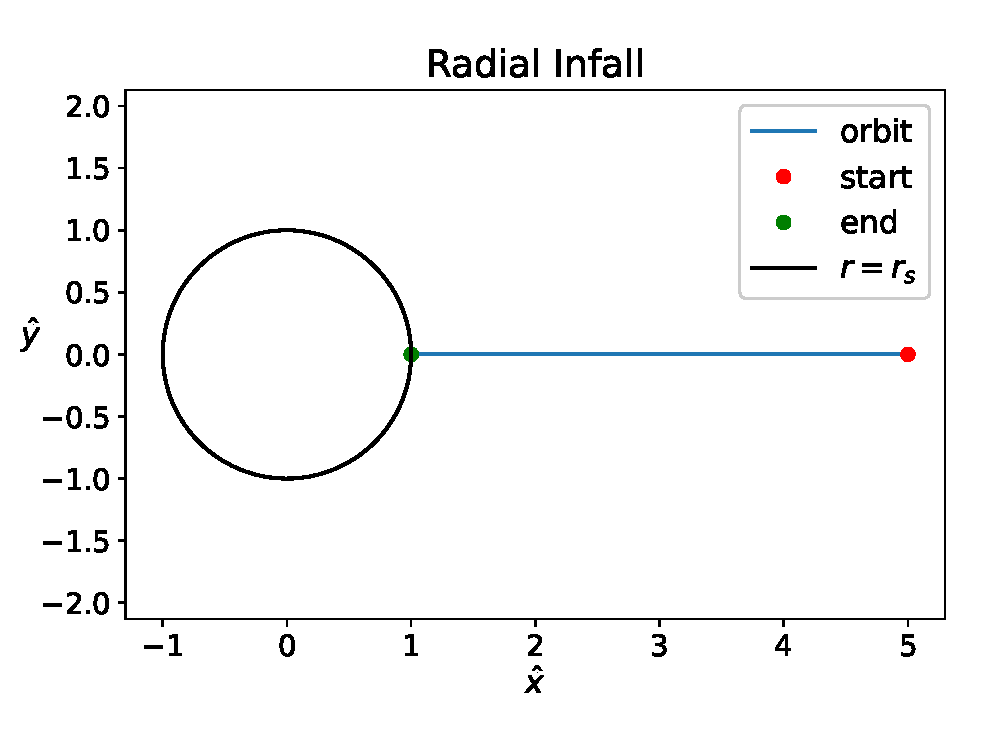
\includegraphics[width=\textwidth]{Figures/ch2/radial_infall.eps}
        \end{minipage}
        \hspace{0.015 \textwidth}
        \begin{minipage}{0.48\textwidth}
            \centering
            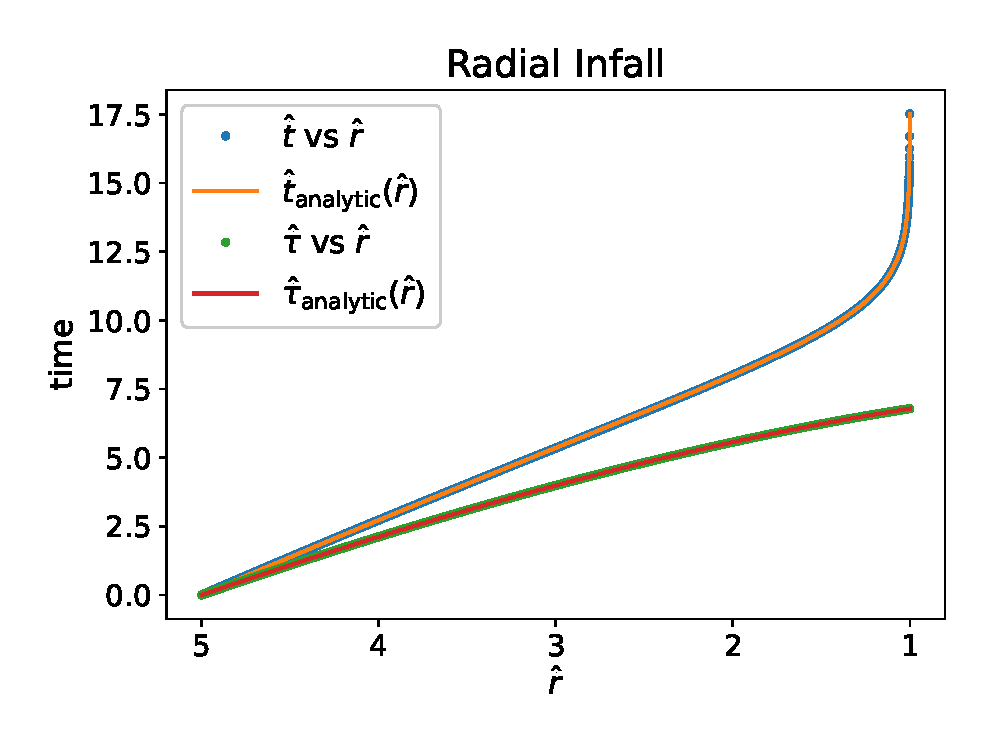
\includegraphics[width=\textwidth]{Figures/ch2/t_vs_tau.eps}
        \end{minipage}
    \end{figure}

\end{frame}


\begin{frame}{Caduta Radiale: Residui}

    $\hat \ell = 0$, $\mathcal E = 0$, $r_0 = 5$, $h = 10^{-4}$ \\
    Prompt: \texttt{./main.x 0 0 -r 5 -h 1e-4}

    \begin{figure}[h]
        \begin{minipage}{0.48\textwidth}
            \centering
            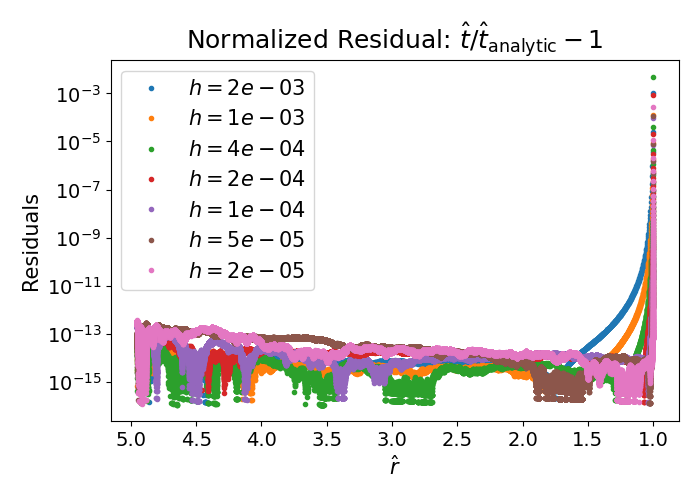
\includegraphics[width=\textwidth]{Figures/ch2/t_res_multi.png}
        \end{minipage}
        \hspace{0.015 \textwidth}
        \begin{minipage}{0.48\textwidth}
            \centering
            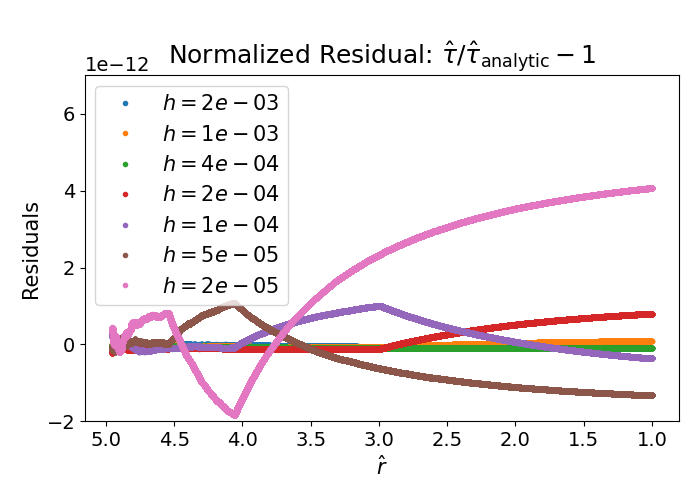
\includegraphics[width=\textwidth]{Figures/ch2/tau_res_multi.png}
        \end{minipage}
    \end{figure}

\end{frame}


\begin{frame}{Caduta $\hat l = 4$, $\mathcal E = 0.85993$}
    \centering
    \movie[externalviewer]{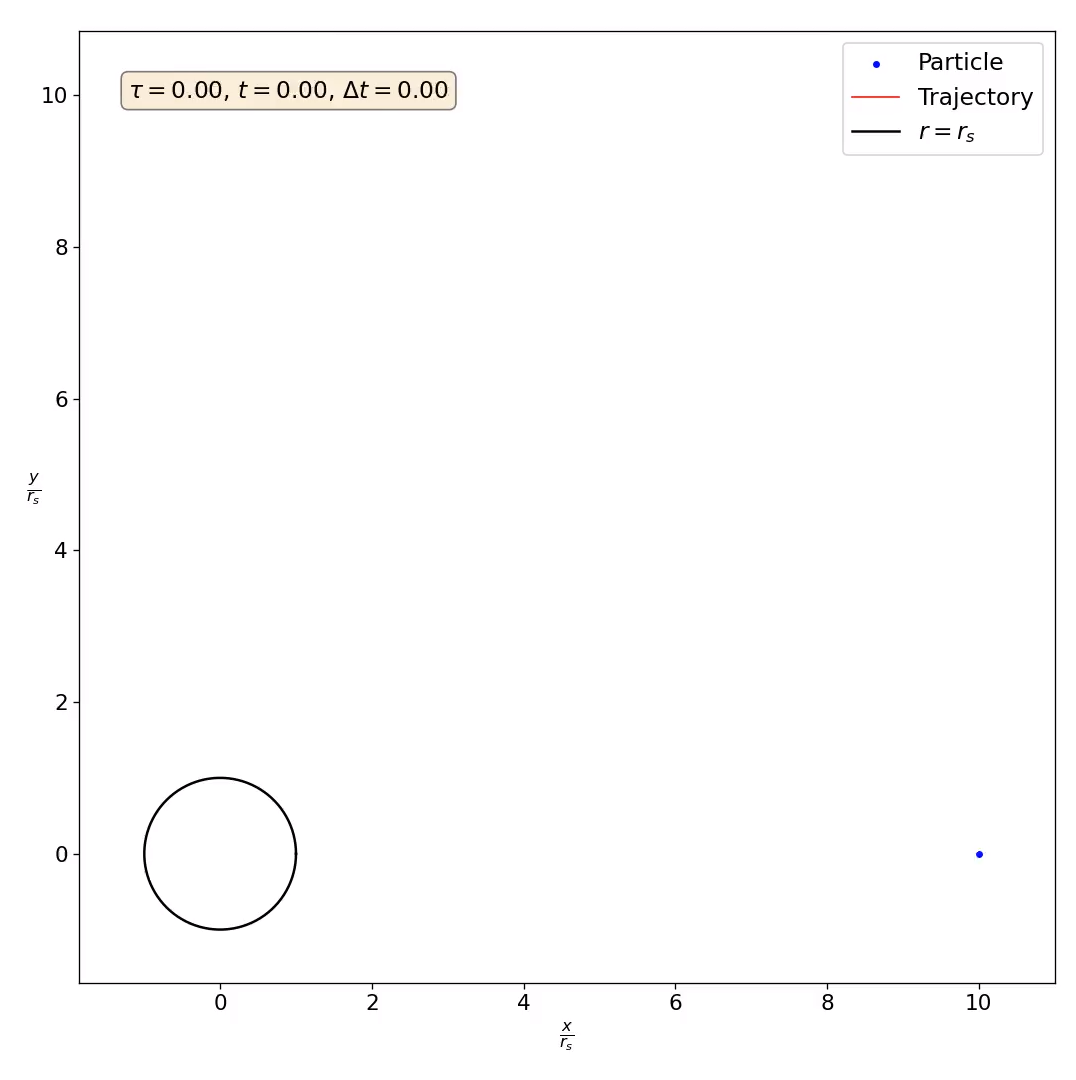
\includegraphics[width=0.6\textwidth]
    {Videos/infall.png}}{Videos/infall_ani.mov}
\end{frame}


\begin{frame}[t,fragile]{Il Cambio di Segno}

    \begin{equation*}
        \dv{\hat r}{\hat \tau} = \pm \sqrt{2 \mathcal E - 2 V_{\rm eff}}
    \end{equation*}

    \vspace{0.5cm}

\begin{lstlisting}[language=C]
double TESI_fun_r(double r, double E, double l, int *sign, int *Nturns){
    double foo = 2 * (E - TESI_Veff(r, l));
    if (foo < 0){
        *sign *= -1;
        *Nturns += 1;
    }
    return *sign * pow(fabs(foo), 1. / 2.);
}
\end{lstlisting}

\end{frame}


\begin{frame}{Casi Possibili, Scelta di $r_0$ e Segno}

    \begin{figure}
        \centering
        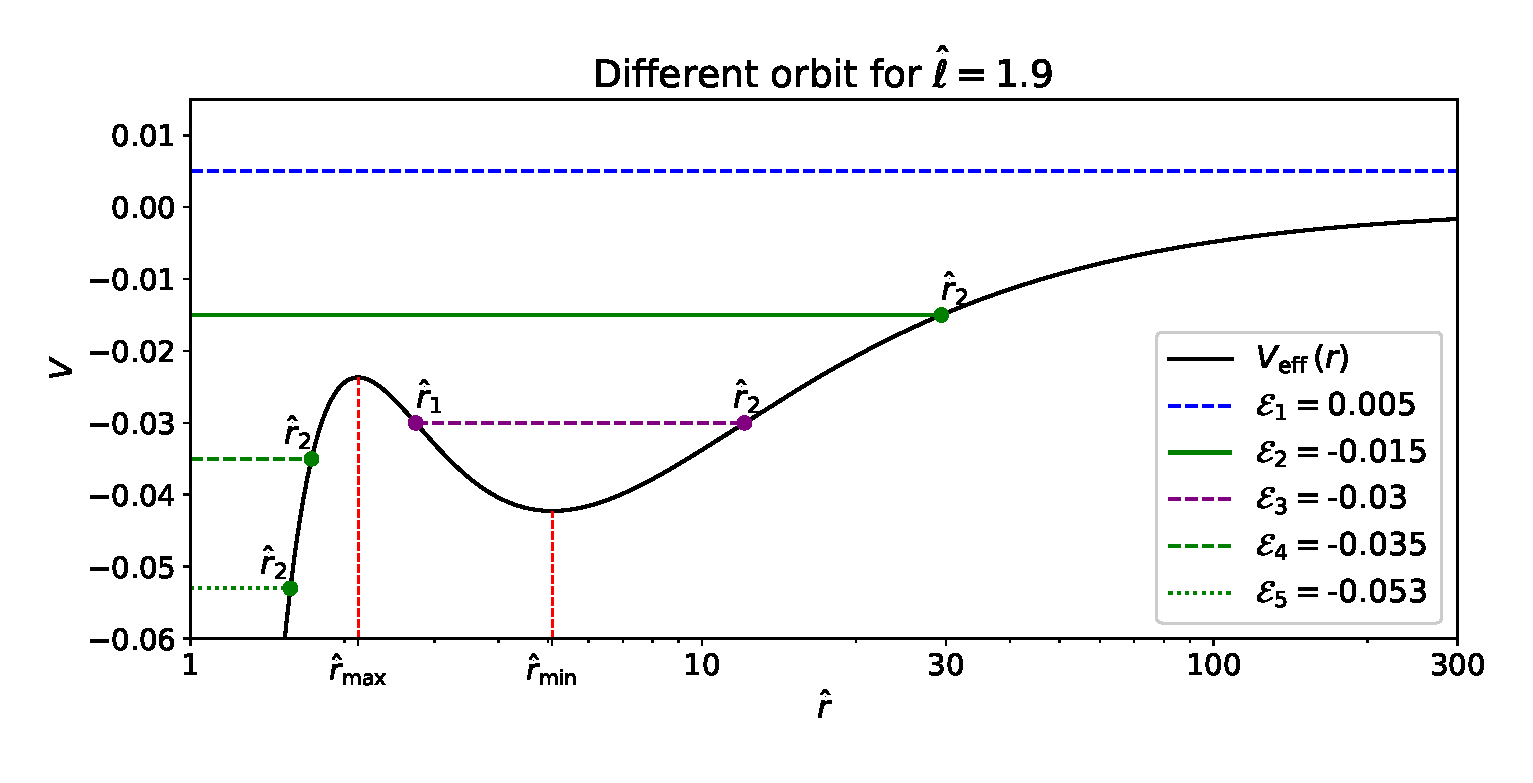
\includegraphics[width=0.9\textwidth]{Figures/ch2/scenario1.eps}
    \end{figure}

\end{frame}


\begin{frame}{Caduta $\hat l = 4$, $\mathcal E = 0.85993$}
    \centering
    \movie[externalviewer]{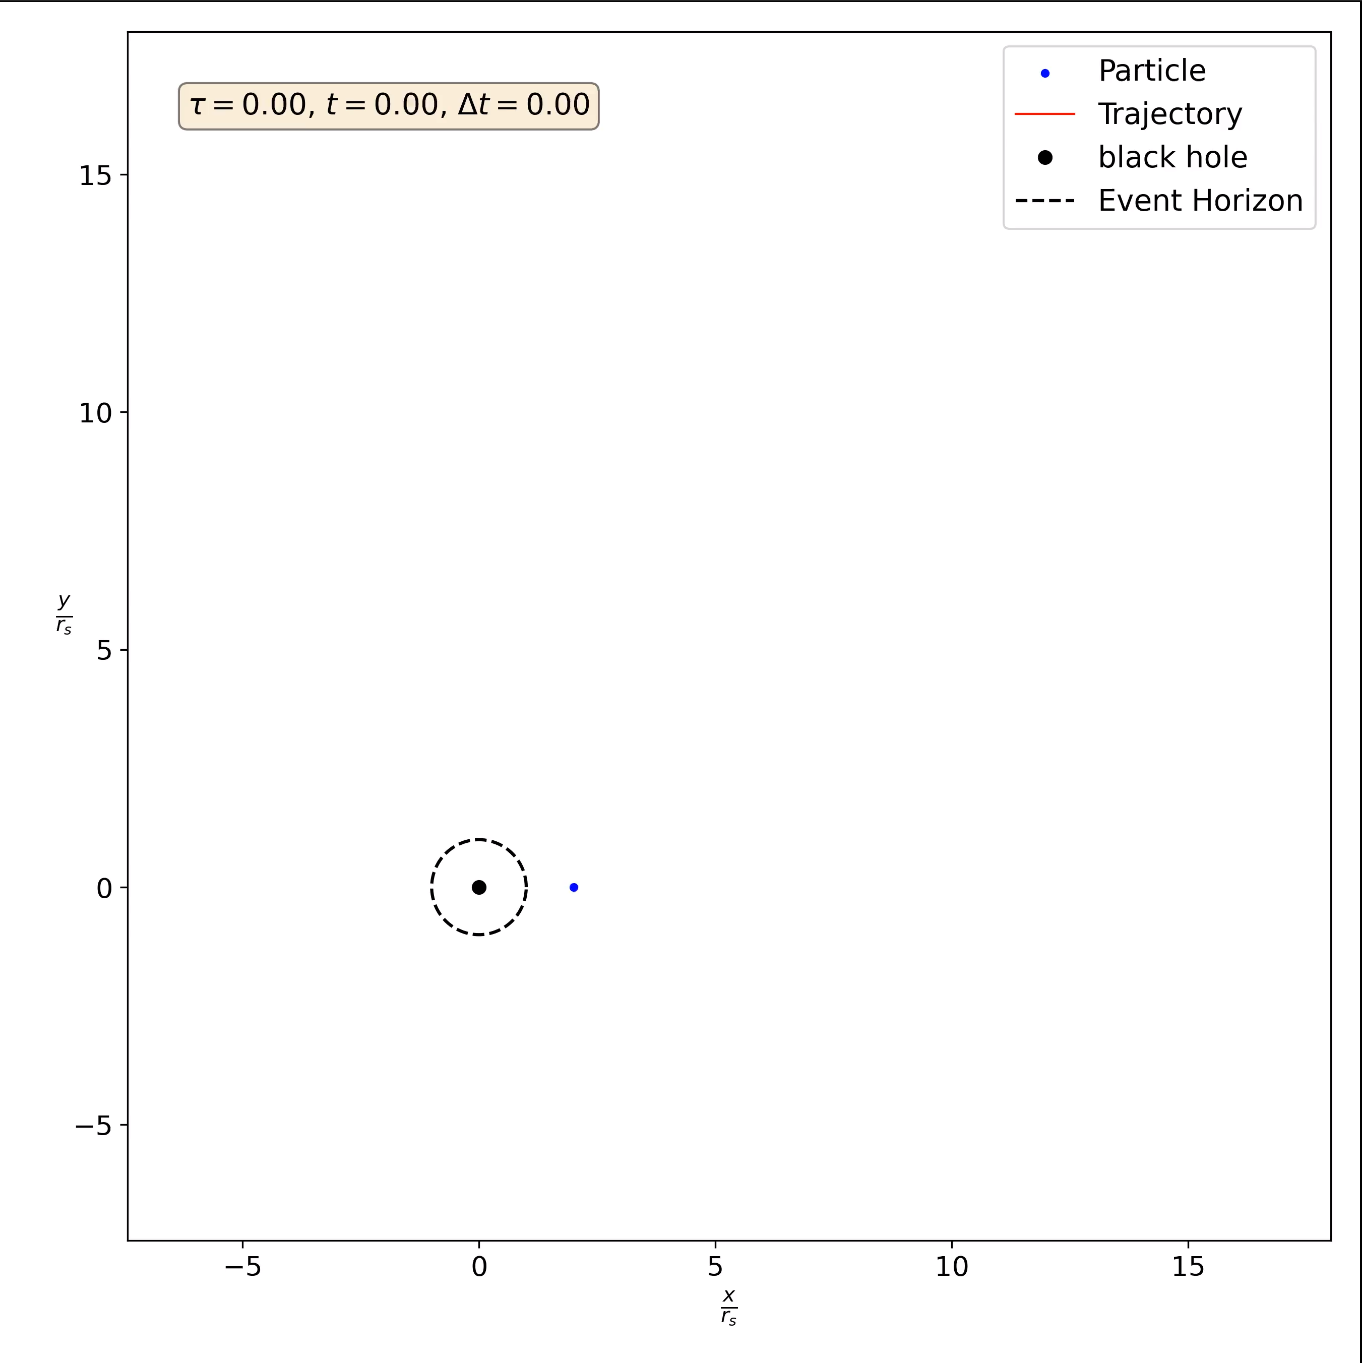
\includegraphics[width=0.6\textwidth]
    {Videos/volevi.png}}{Videos/volevi_ani.mov}
\end{frame}


\begin{frame}{Test di Stabilità}
    \begin{figure}
        \centering
        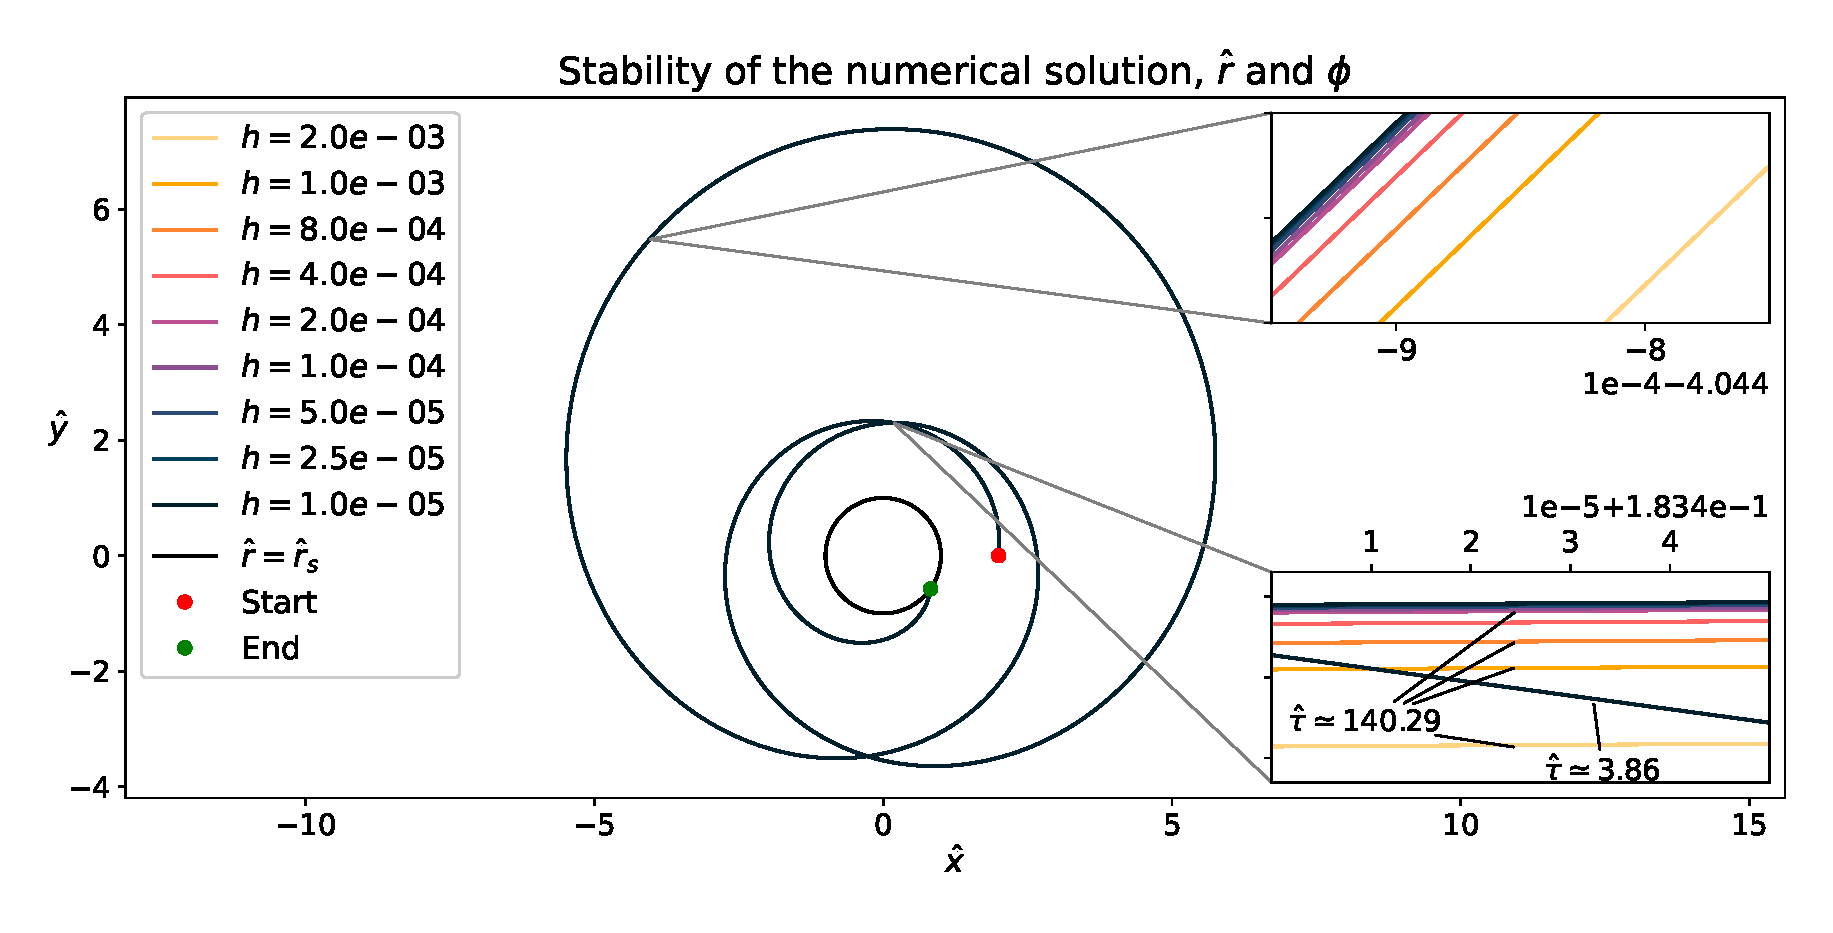
\includegraphics[trim={0 0 0 37},clip, width=\textwidth]{Figures/ch2/stability_infall2.eps}
        \caption{ $\hat \ell = 1.8$, $\mathcal E = -0.042$, $\hat r_0 = 2$}
    \end{figure}
\end{frame}


%\begin{frame}{Casi Possibili, Scelta di $r_0$ e Segno}
%
%    \begin{figure}
%        \centering
%        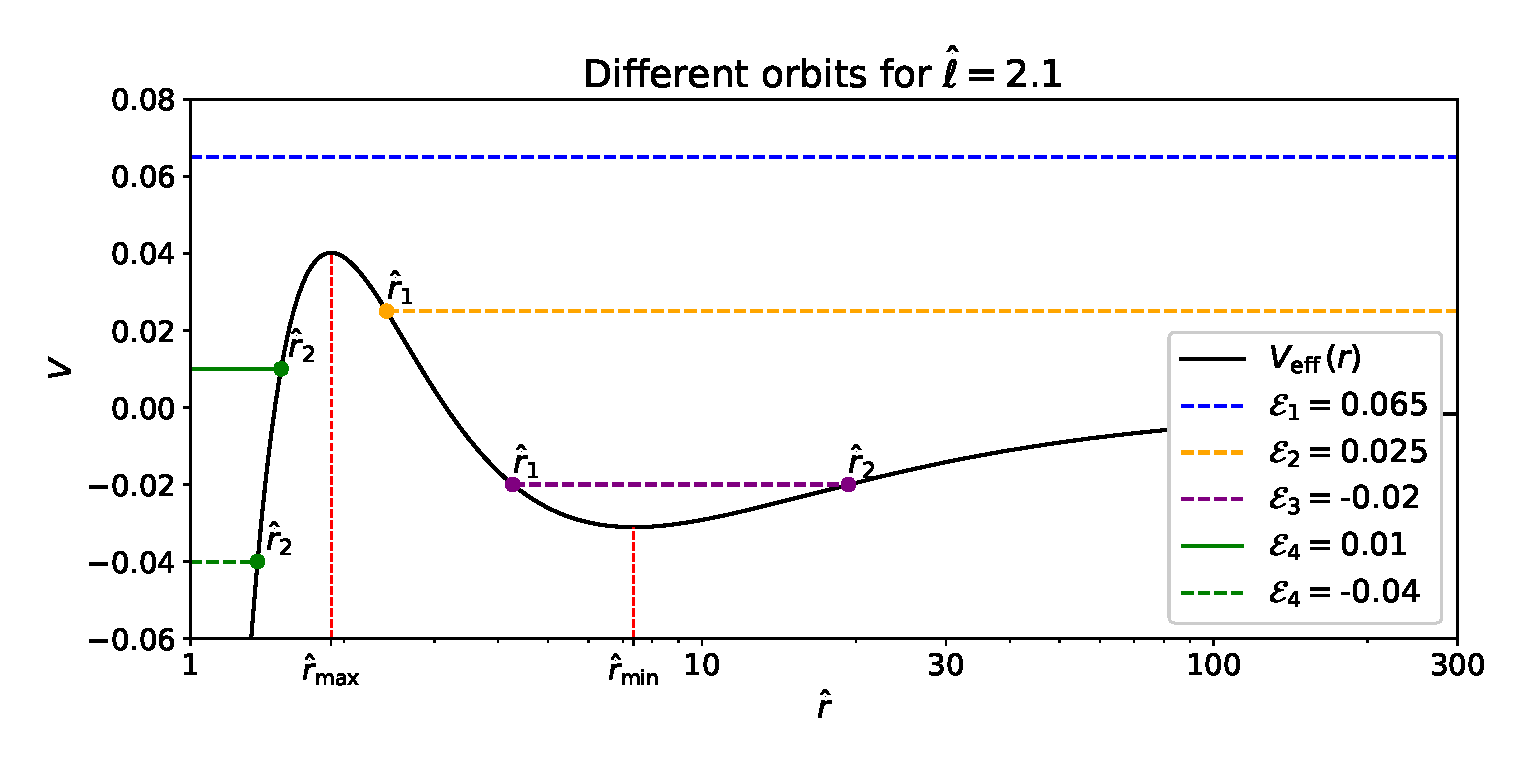
\includegraphics[width=0.9\textwidth]{Figures/ch2/scenario2.eps}
%    \end{figure}
%
%\end{frame}


\begin{frame}{Precessione di Orbite Stabili}
    \centering
    \movie[externalviewer]{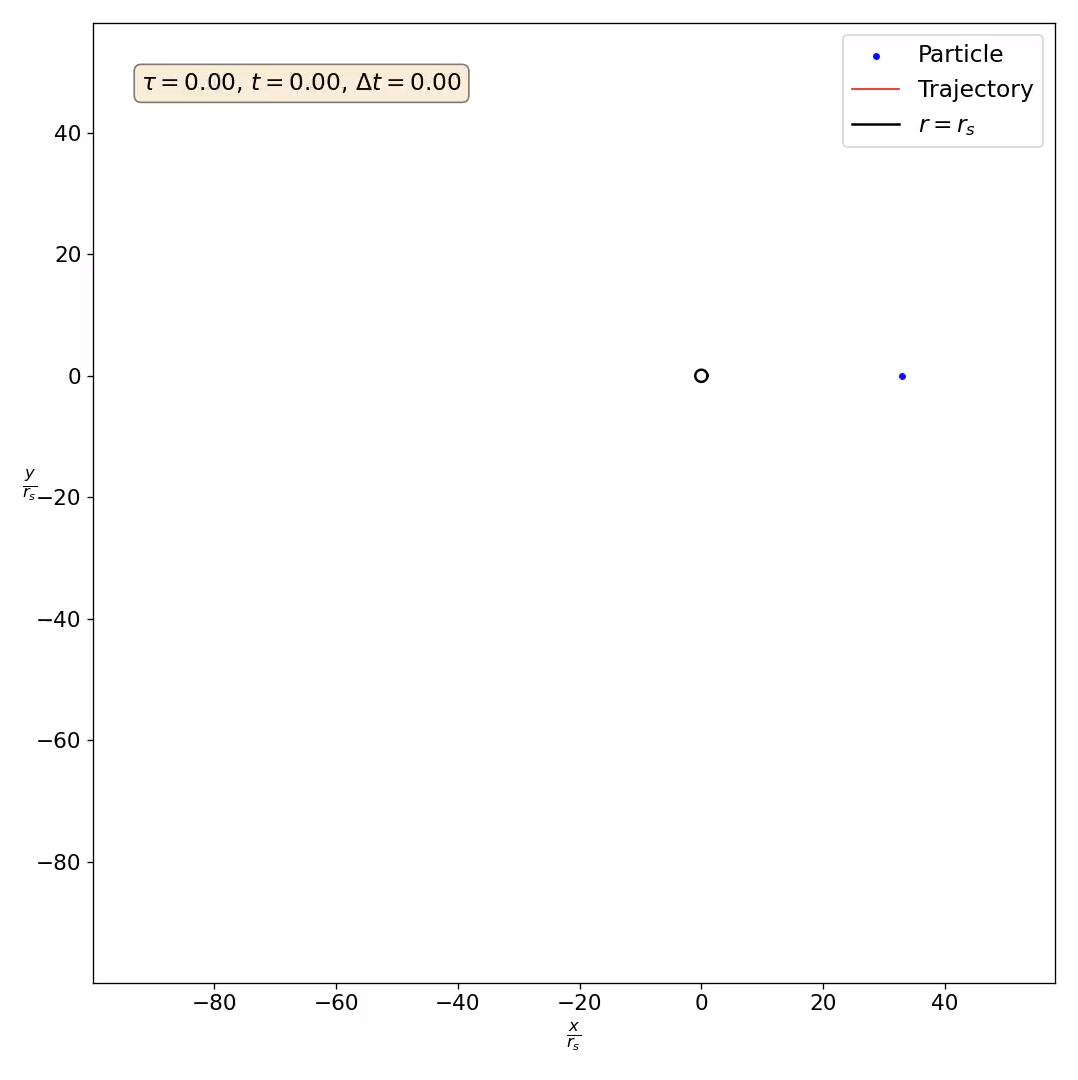
\includegraphics[width=\textheight, keepaspectratio]
    {Videos/prec1.png}}{Videos/prec1_ani.mov}
\end{frame}


\begin{frame}{Precessione: Simulazione e Valore Teorico}
    \begin{figure}[h]
        \centering
        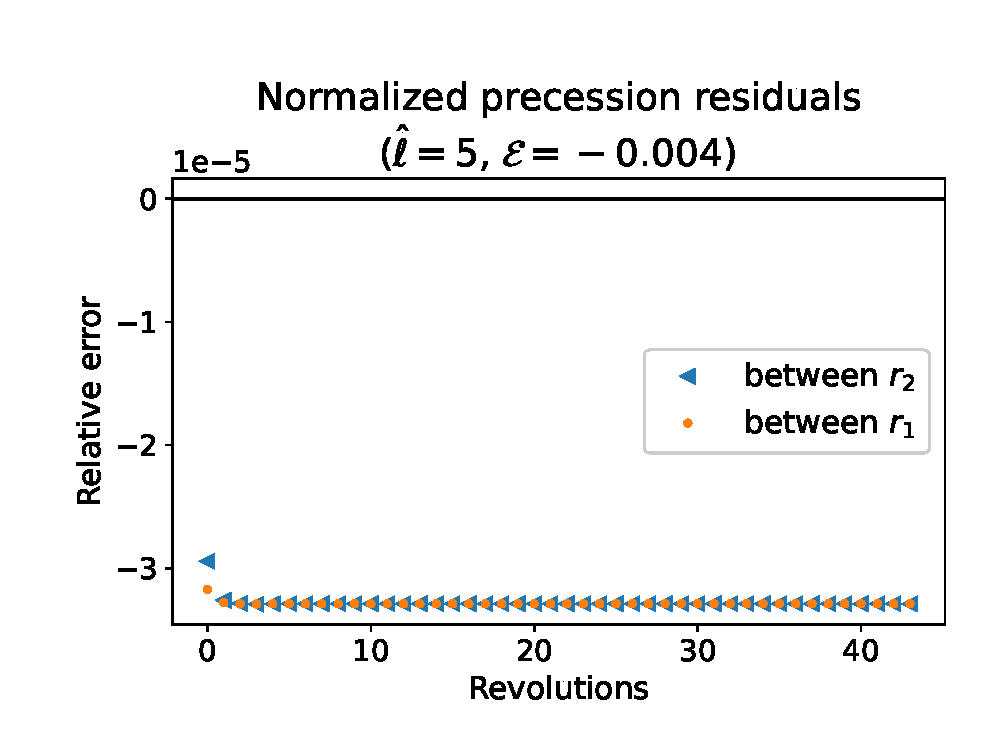
\includegraphics[width=0.7\textwidth]{Figures/ch2/prec1_res.eps}
        \caption{$\hat \ell = 5$, $\mathcal E = -0.004$, $\hat r_0 = r_1
        \simeq 32.9$, evolved for $\hat \tau = \num{1.2e5}$.
        $\delta \phi_{\rm theory} \simeq 0.0652 \pi$, $\delta \phi_{\rm avg}
        = \delta \phi_{\rm theory} - \num{7e-6} \pm \num{2e-8}$.}
    \end{figure}
\end{frame}


\begin{frame}{Precessione di Orbite Stabili}
    \centering
    \movie[externalviewer]{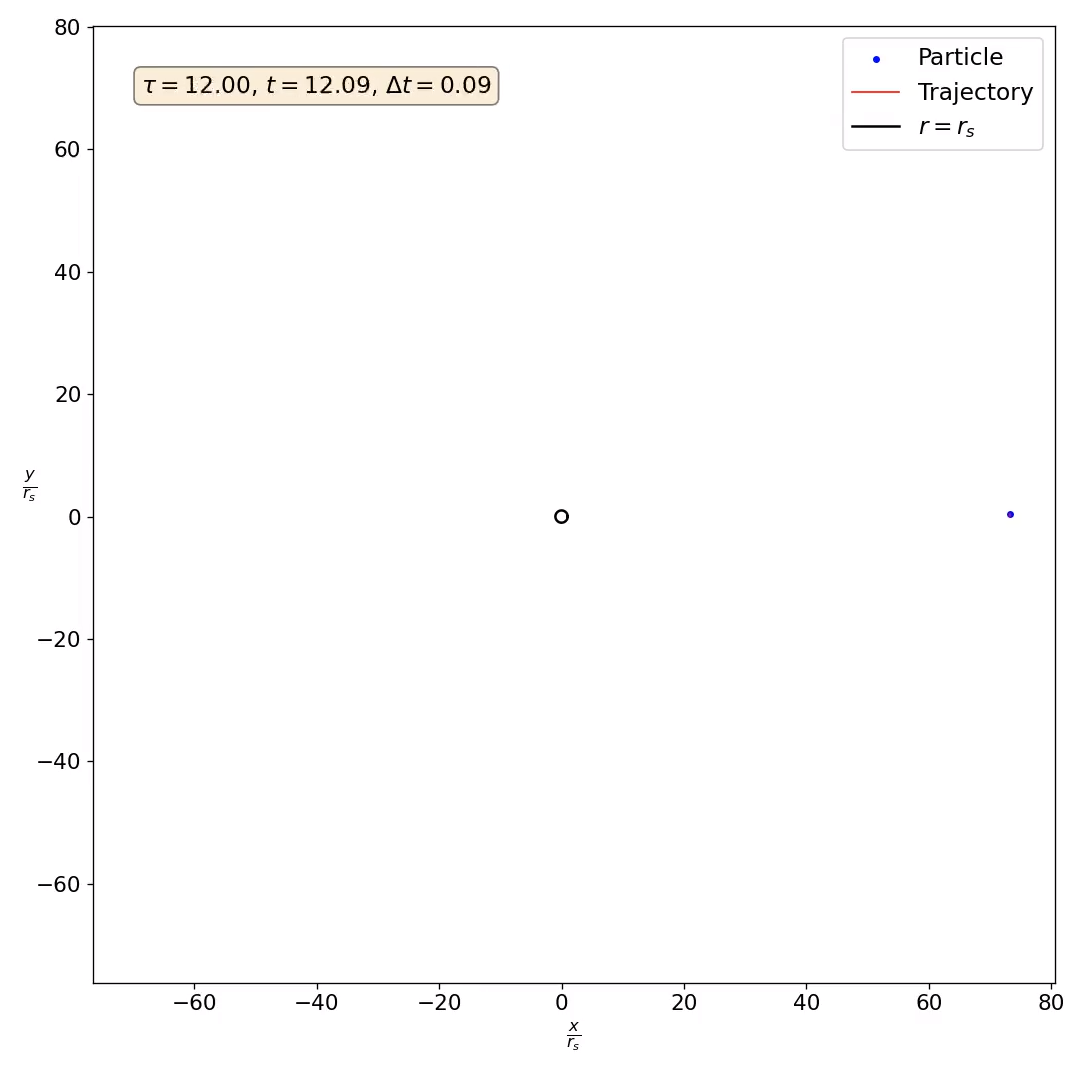
\includegraphics[width=0.8\textheight, keepaspectratio]
    {Videos/prec2.png}}{Videos/prec2_ani.mov}
\end{frame}


\begin{frame}{Precessione: Simulazione e Valore Teorico}

    Invece di utilizzare

    \begin{equation*}
       \dv{\hat r}{\hat \tau} = \pm \sqrt{2 \mathcal E - 2 V_{\rm eff}}
    \end{equation*}

    Definiamo:

    \begin{align*}[left = {\empheqlbrace}]
        &\dv{\hat v}{\hat \tau} = - \dv{V_{\rm eff}}{\hat r} 
        = \frac{\hat \ell^2}{\hat r^3} - \frac{1}{2 r^2}
        - \frac{3 \hat \ell^2}{2 \hat r^4} \\
        &\dv{\hat r}{\hat \tau} = \hat v \\
        &\dv{\phi}{\hat \tau} = \frac{\hat \ell}{\hat r^2} \\
        &\dv{t}{\hat \tau} = \sqrt{2 \mathcal E + 1}
        \left(\frac{\hat r}{\hat r - 1}\right)
    \end{align*}
\end{frame}


\begin{frame}{Precessione: Simulazione con Metodo Alternativo}

    \begin{figure}[h]
        \centering
        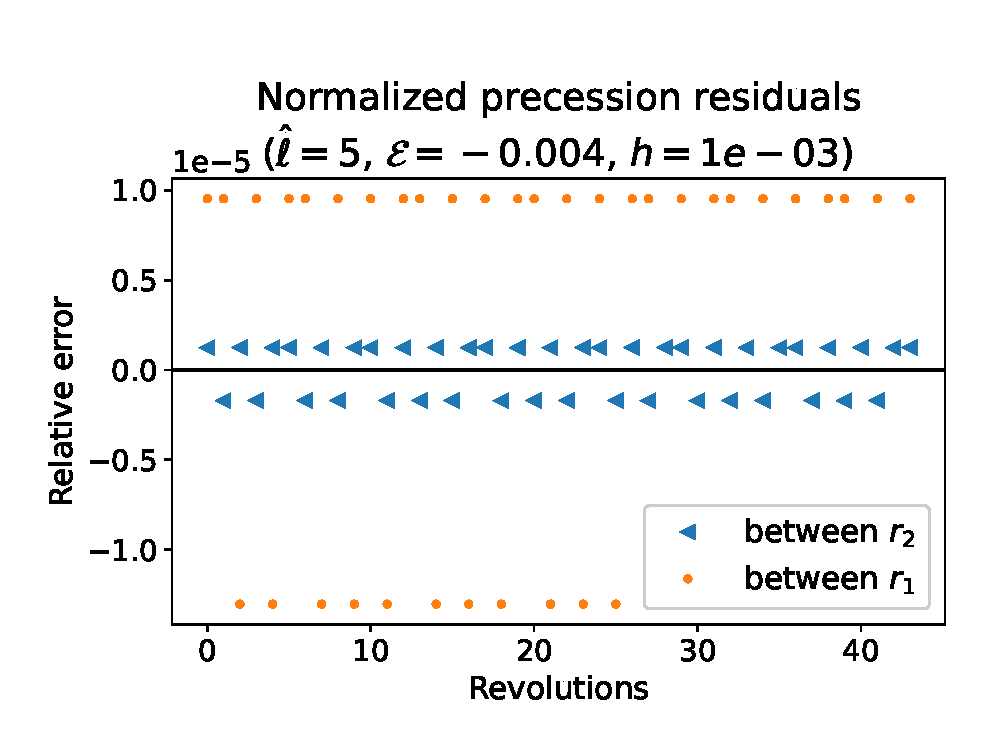
\includegraphics[width=0.7\textwidth]{Figures/ch2/prec1_res_corr.eps}
        \caption{$\hat \ell = 5$, $\mathcal E = -0.004$, $\hat r_0 = r_1
        \simeq 32.9$, evolved for $\hat \tau = \num{1.2e5}$.
        $\delta \phi_{\rm theory} \simeq 0.0652 \pi$, 
        $\delta \phi_{\rm avg} = \delta \phi_{\rm theory} + (8 \pm 40) \times 
        \num{e-9}$.}
    \end{figure}

\end{frame}


